\chapter{\eloismeretek}

\section{Esettanulmány}
A dolgozatban elért eredményeket a Train Benchmark \cite{szarnyas2018train} esettanulmány segítségével fogom bemutatni. Ez a benchmark azért jött létre, hogy össze tudjuk hasonlítani különböző gráflekérdező rendszerek teljesítményét, beleértve gráfadatbázisokat, mint Neo4j \cite{neo4j},  SparkSee \cite{sparksee}, nagy teljesítményű modellezőeszközöket, mint VIATRA \cite{viatra} és szokványos relációs adatbázisokat, mint az Oracle \cite{oracle}, főleg időigény és memória felhasználás szempontjából. A Train Benchmark egy vasúti modellezőeszköz esettanulmányán mutat be olyan, különböző terhelésprofilokat, amelyek hasonlítanak egy valódi modellezési feladathoz. Munkám során a benchmarkban specifikált formátumhoz illeszkedve generáltam lekérdezéseimet, ezért bemutatom, hogy milyen elemekből áll. 

\begin{figure}
	\centering
	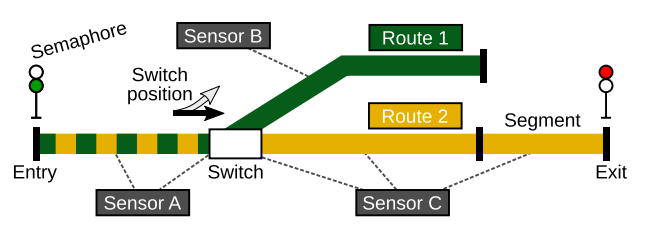
\includegraphics[width=0.7\textwidth]{figures/trainbenchmarkfig1}
	\caption{Vasúti útvonal részlet (forrás: \cite{szarnyas2018train})}
	\label{fig:trainbenchmark}
\end{figure}

\Aref{fig:trainbenchmark}-es ábrán látható egy a Train Benchmark modelljére alapuló részlet.
Ebben a kontextusban egy vasúti útvonal(\textit{Route}, zölddel és sárgával jelölve) nem más mint szegmensek(\textit{Segment}, két fekete vonal közötti rész) és váltók (\textit{Switch}, fehér téglalappal jelölve) sorozata, illetve a belépést és a kilépést egy-egy szemafor(\textit{Semaphore}, a két színű lámpácskák jelölik) jelzi. Ahhoz, hogy biztonságos legyen a közlekedés szükség van szenzorokra, amelyek monitorozzák a különböző szegmensek és váltók kihasználtságát. Egy útvonal definiálásához, a felsorolt elemeken kívül a váltók adott útvonalhoz tartozó pozícióját is el kell tárolnunk. Egy útvonal akkor aktív, ha a rendszerben a specifikációjának megfelelően állnak a váltók.




\section{Gráflekérdező rendszerek}
\subsection{Tulajdonság gráfok}

A gráfok intuitív formalizációt nyújtanak modellezési szempontból arra, hogy úgy írhassuk le a világot ahogy az ember gondolkozik róla. Tehát mint dolgok (csomópontok) és köztük lévő kapcsolatok (élek)\cite{marton2017model}. A tulajdonsággráf (property graph) adatmodell kiterjeszti a gráfokat úgy, hogy címkéket/típusokat, illetve tulajdonságokat ad a csúcsoknak és az éleknek. A gráf adatbázisok  alkalmasak tulajdonsággráfok tárolására, és az abban lévő adatok lekérdezésére komplex gráf minták használatával. Ilyen rendszerek például a Neo4j \cite{neo4j}, OrientDB \cite{orientdb} és a  SparkSee \cite{sparksee}.

\begin{figure}
	\centering
	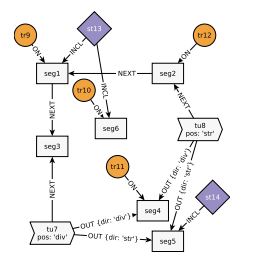
\includegraphics[width=0.6\textwidth]{figures/tulajdonsággráfpélda}
	\caption{Tulajdonsággráf példa(forrás: \cite{marton2017model})}
	\label{fig:tulajdonsággráfpélda}
\end{figure}

Ahhoz hogy jobban megérthessük mi is ez az adatmodell \aref{fig:tulajdonsággráfpélda} -es ábrán látható egy példa. Az ábrán minden ami valamilyen forma egy-egy csomópont, és minden csomópont reprezentál elemeket a Train Benchmark adatmodelljéből. A fehér téglalapok a szegmenseket,  a sárga körök a vonatokat, a lila rombuszok az útvonalakat, és a fehér zászlók a váltókat. Minden elem fel van címkézve ezen kívül egy névvel (seg1, seg2, tr1 stb...), a formájuk és a nevük is tulajdonságok amelyek segítségével megkülönböztethetővé válnak,és amelyek egy egyszerű gráfban már nem lehetnének jelen. Az élek pedig kapcsolatokat mutatnak az egyes elemek között. Például az ábrán vannak összekötött vonatok és szegmensek, az összekötő élen "ON" felirattal. A vonattól mutatnak a szegmens irányába. Egy ilyen irányított él azt reprezentálja, hogy az adott vonat rajta van az adott szegmensen(angolul : train is ON segment). Ilyen formán az élekhez is rendelhetőek tulajdonságok. 


 
 
\subsection{Neo4j}

A Neo4J egy népszerű NoSQL tulajdonsággráf adatbázis és a Cypher lekérdező nyelvet kínálja lekérdezések írására. A Cypher egy magas szintű deklaratív lekérdező nyelv és mivel le van választava a lekérdező rendszerről, ezért az képes a Cypher nyelven írt lekérdezések optimalizálására. A Cypher szintaxisa olyan gráf minták megírását teszi lehetővé, amelyeknek megértése nagyon egyszerű.


\begin{lstlisting}[style=cyphersmall]
MATCH (tr:Train)-[:ON]->(seg:Segment)
RETURN tr, seg	
\end{lstlisting}   

A fenti példán egy olyan lekérdezést láthatunk,  ami az összes olyan vonat, szegmens párral tér vissza, ahol az adott vonat rajta van az adott szegmensen.  Dolgozatomban Cypher nyelvű lekérdezések generálásával foglalkozom.

Egy Cypher nyelvű lekérdezésben a \cypherStyle{MATCH} kikötést arra használjuk hogy megkeresse a mintát amit leírunk benne.
A \cypherStyle{RETURN} kikötés meghatározza hogy mi kerüljön bele a visszatérési értékbe. () zárójelek között változókat definiálunk és meghatározhatjuk a címéjüket is például (tr:Train) a tr a változó neve, ami Train típusú. {} zárójelek között ezután további tulajdonságokat köthetünk ki. --> jelöli a kapcsolatot két változó között, ahol a két kötőjel között [] zárójelekben megadható a kapcsolatra vonatkozó címke. 

A Neo4j képes arra hogy egy ilyen lekérdezést beolvasson, és kiértékeljen majd visszatérjen a lekérdezésre adott válaszokkal. Azonban, mint minden szoftver a lekérdező rendszerek is tartalmaznak hibákat,amelyek következtében hibás kimeneteket adnak a lekérdezések eredményeként. Ezért a lekérdező rendszerek tesztelése kiemelten fontos.

\section{Modellezés és metamodellezés}

A metamodellezés egy tecknika arra, hogy definiáljunk új modellező nyelveket. A Train Benchmark metamodellje \aref{fig:trainbenchmarkmetamodell} -es ábrán látható.

A céldomén legfontosabb fogalmait és kapcsolatait foglalja össze a metamodell, így specifikálva a modellek alap struktúráját \cite{semerath2017formal}. Dolgozatomban az Eclipse Modeling Framework (EMF) \cite{EMF} -öt használtam metamodellezésre. EMF esetén a fogalmakat osztályokkal (EClass) a kapcsolatokat referenciákkal és attribútumokkal (EReference és EAttribute) írjuk le.

\begin{figure}
	\centering
	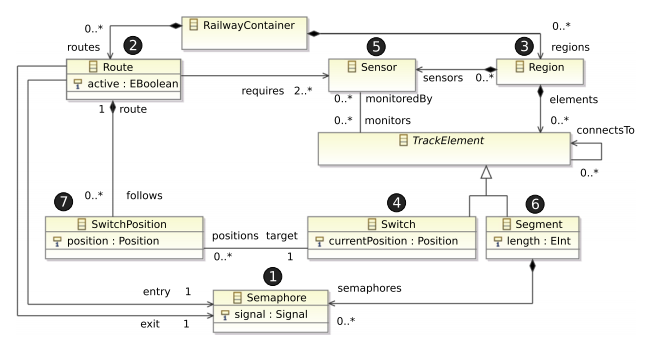
\includegraphics[width=0.7\textwidth]{figures/trainbenchmarkfig2}
	\caption{A Train Benchmark metamodellje.(forrás: \cite{szarnyas2018train})}
	\label{fig:trainbenchmarkmetamodell}
\end{figure}

\subsection{Cypher query-k metamodellje}

\Aref{fig:cyphermetamodell} -ös ábrán látható a korábban említett Cypher nyelv egyszerűsített metamodellje.
A \viatraStyle{SinglePartQuery} elem reprezentálja a modell gyökerét. Egy ilyen elem két részből áll : Egy \viatraStyle{Match} 
és egy \viatraStyle{Return} elemből. A \viatraStyle{Match} elem minták összességéből áll (\viatraStyle{Pattern}), amelyek 
részekre (\viatraStyle{PatternPart}) bonthatóak. Egy ilyen részben pedig vagy tartalmaz változó deklarációt,
vagy egy belső részt, ami tartalmaz változó deklarációt. (\viatraStyle{VariableDeclaration}).
Ezáltal az összes változót a \viatraStyle{Match} elemen belül deklaráljuk. A \viatraStyle{Return} elem  pedig egy
kifejezést (\viatraStyle{Expression}) tartalmaz, amelyben mindenképp szerepel egy változó referencia
 (\viatraStyle{VariableRef}) is, így összekötve egymással a \viatraStyle{Match} és a \viatraStyle{Return} elemet. 

\begin{figure}
	\centering
	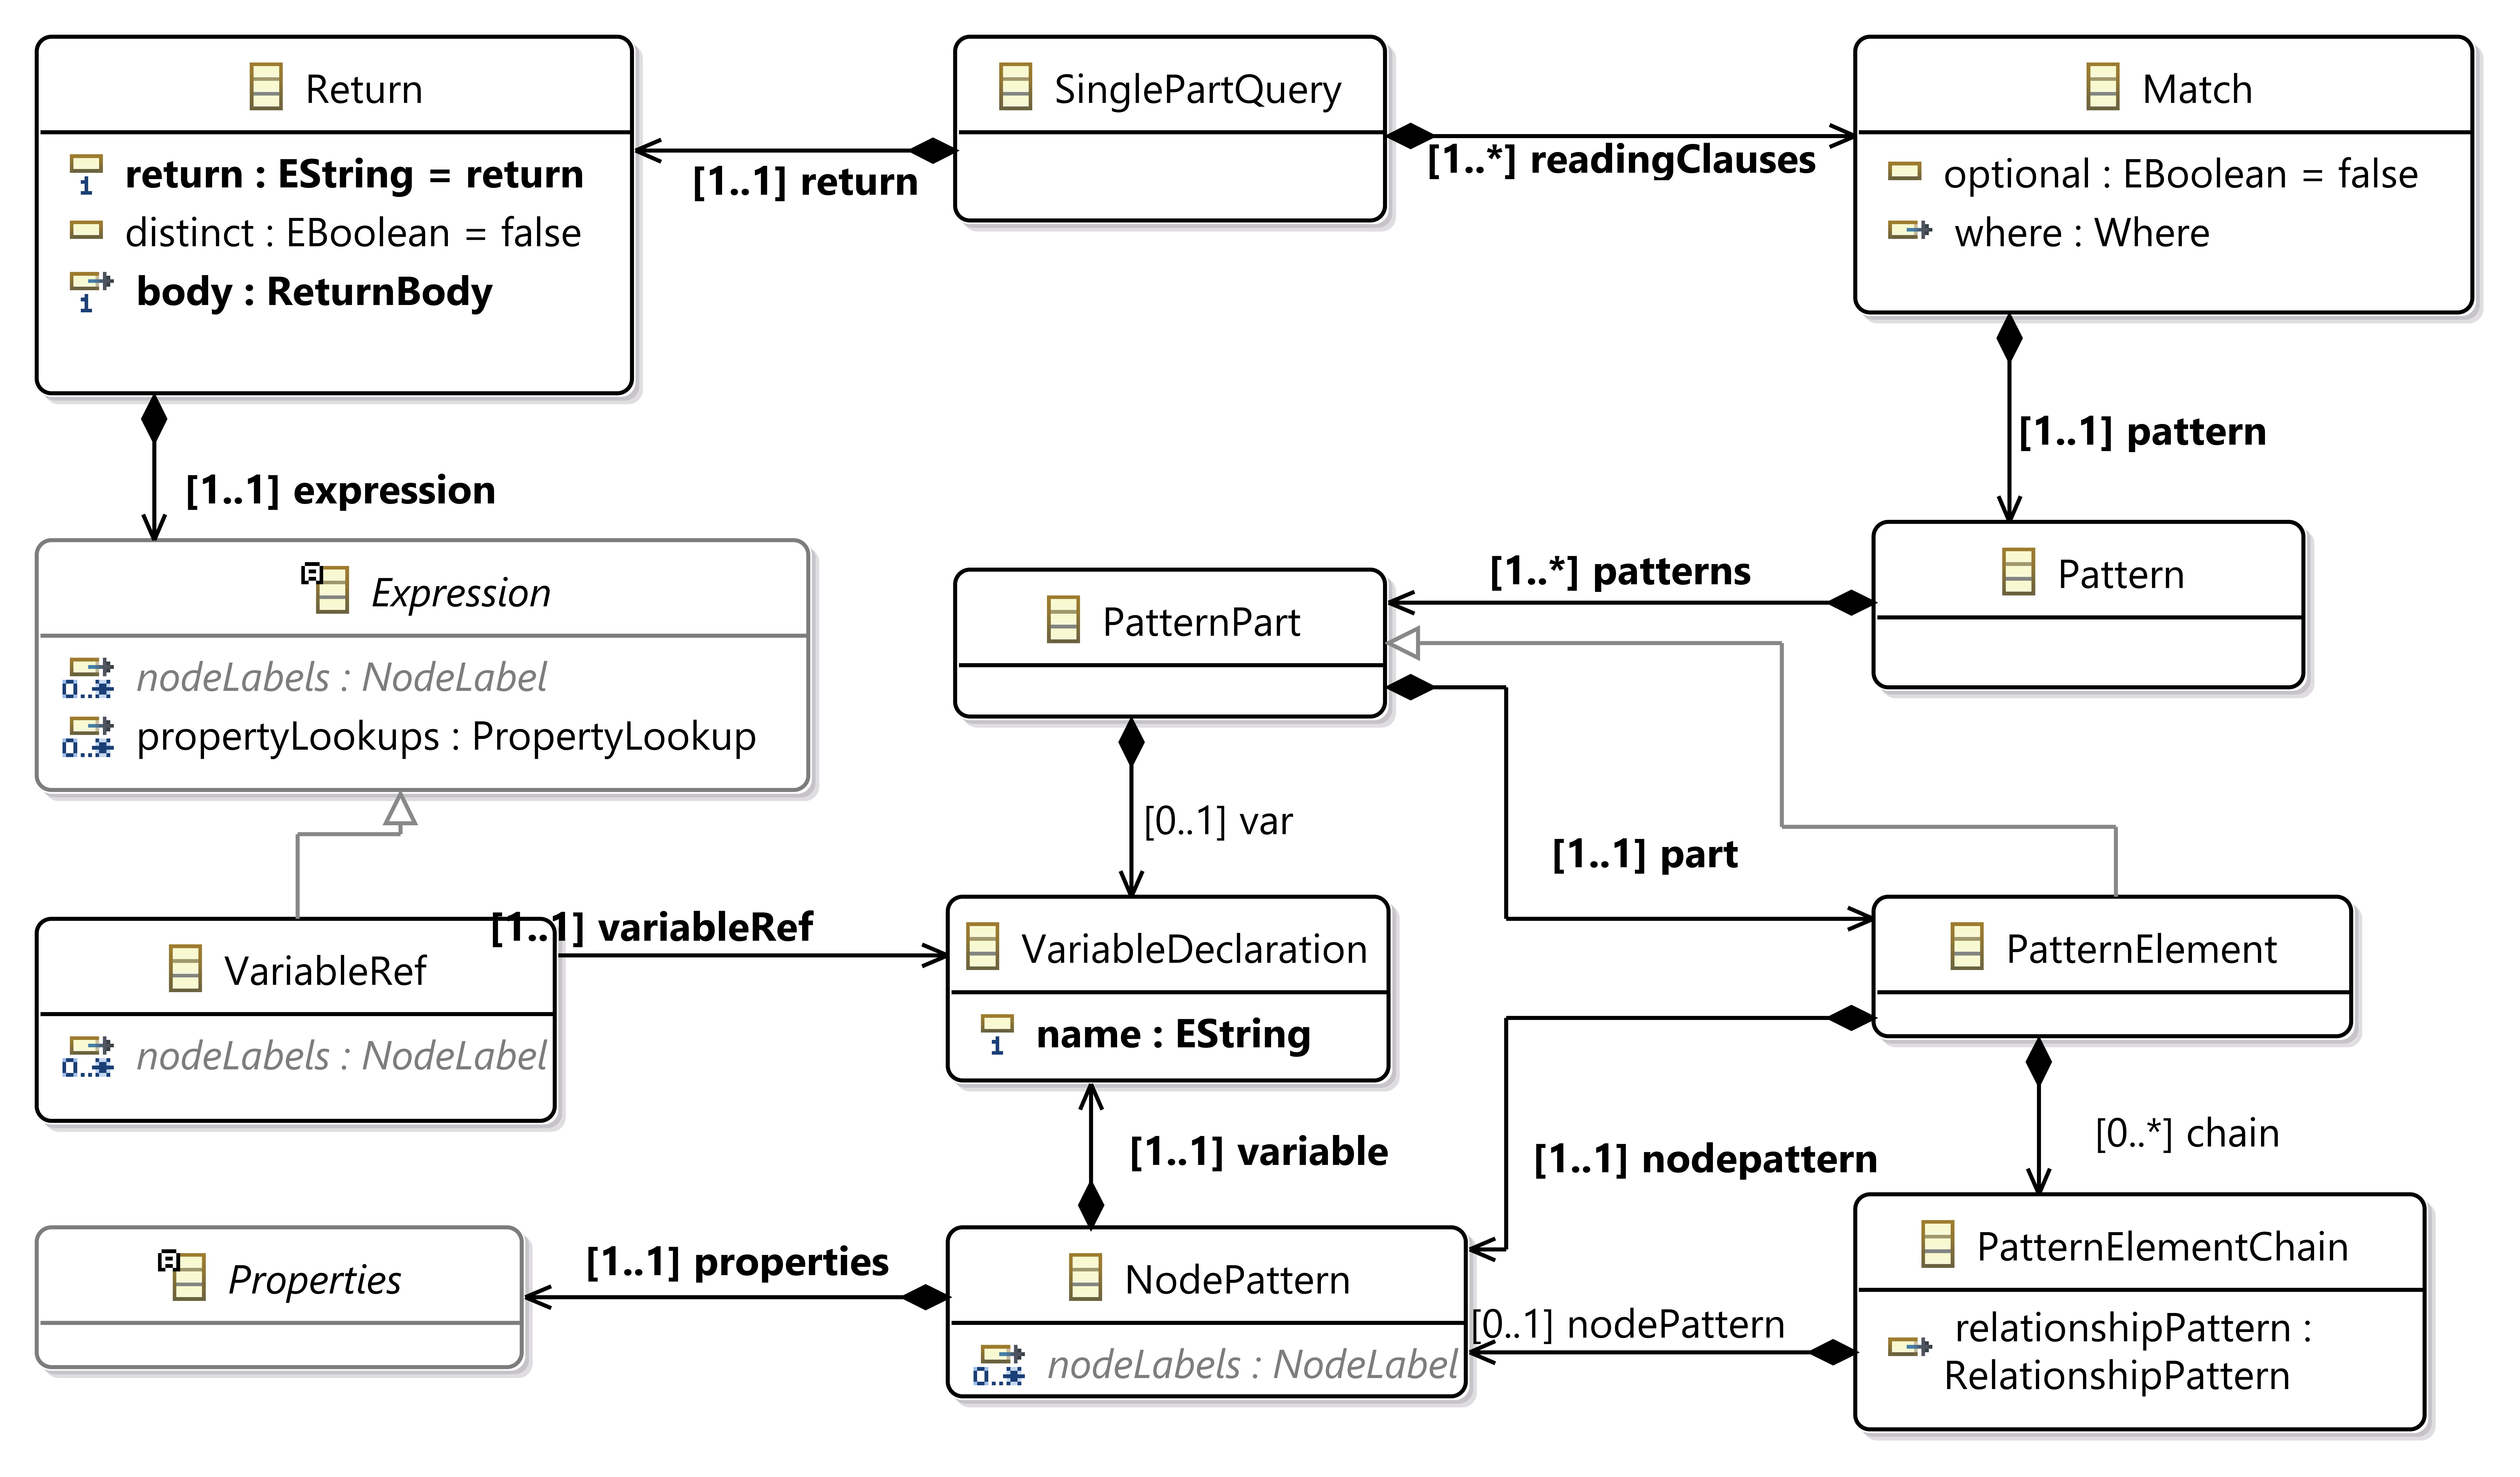
\includegraphics[width=0.7\textwidth]{figures/openCypherClassDiagram}
	\caption{Cypher metamodell}
	\label{fig:cyphermetamodell}
\end{figure}


\subsection{Xtext}

Az Xtext keretrendszer programozási nyelvek,  domain-specifikus nyelvek és szöveges editorok fejlesztésére készül. Az Xtext  
egy erős nyelvtani szabályokkal rendelkező nyelvet használ az egyedi nyelvtanok definiálására. Ezáltal
egyszerre biztosít parseolót, linkelőt, helyesírásellenőrzőt szövegkiemelést, hibaüzeneteket és  írás során könnyen kiegészíthető fordítókkal, kódgenerátorokkal és egyéb modellezőeszközökkel. És a nyelvtervező mérnök határozhatja meg a nyelvének célformátumát is. Ahhoz, hogy a Cypher nyelven megírt lekérdezéseket értelmezni lehessen 
\aref{fig:cyphermetamodell}-ös metamodellen megismert elemek szintjén egy Xtext \cite{xText} keretrendszerben íródott nyelvtanra van szükség, amelyből a metamodell automatikusan elkészült . A dolgozatomban a slizaa\cite{slizaa_2018} nevű Xtext alapú Cypher nyelvtant használtam.

\begin{lstlisting}[style=cyphersmall]
SinglePartQuery:
(readingClauses+=ReadingClause)* return=Return ;

Return:
(return='RETURN' distinct?='DISTINCT'? body=ReturnBody);

ReadingClause:
LoadCSV | Start | Match | Unwind | InQueryCall;
\end{lstlisting}



A fenti ábrán a SinglePartQuery elem Xtext nyelvtana látható. Azt mondja ki,
hogy amikor egy ilyen elem készül akkor összerak egy vagy több ReadingClause-t (Match elem absztrakt ősosztálya, 3. nyelvtani részlet),
és egy returnt. Alatta pedig a Return elem Xtext nyelvtana következik, ami azt mondja ki hogy a return
elemet úgy kell sorosítani, hogy "\cypherStyle{RETURN DISTINCT}(ezt csak akkor kell odaírni ha ezt a tulajdonságot igazra
állítottuk) \cypherStyle{kifejezes}". Tehát itt határozza meg hogy a Return elem úgy néz ki  mint az alábbi lékérdezésen.

\begin{lstlisting}[style=cyphersmall]
MATCH (tr:Train)-[:ON]->(seg:Segment)
RETURN tr, seg	
\end{lstlisting} 

Ezt a lekérdezést Xtext segítségével ősösztlyaira lehet bontani, és megnézni, mi micsoda benne. Erről \aref{fig:Xtexttelkibontotthelloworld}  ábrán láthatunk egy példát.

\begin{figure}
	\centering
	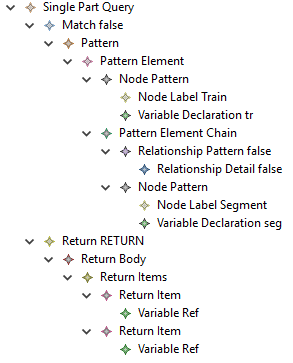
\includegraphics[width=0.5\textwidth]{figures/Xtextelkibontotthellowolrd}
	\caption{A példalekérdezés kibontása Xtext-tel}
	\label{fig:Xtexttelkibontotthelloworld}
\end{figure}


\subsection{\textsc{VIATRA} jólformáltsági kényszerek}
Az Eclipse  \textsc{VIATRA} keretrendszer \cite{viatra} egy modell lekérdező, validáló és transzformációs eszköz. Specifikusan olyan eseményvezérelt
és reaktív transzformációkra fókuszál, amelyek a modell változása közben történnek.  Hibás modellrészletek hibamintákkal történő megfogalmazásával olyan jólformáltsági kényszereket is megadhatunk általa, amelyek kifejezésére a metamodell önmagában nem lenne alkalmas. A lekérdezés generálás során erre használom.


\begin{lstlisting}[style=viatrasmall]

pattern hasMatch (q : SinglePartQuery, m: Match){
	SinglePartQuery.readingClauses(q,m);
}

@Constraint(severity = "error", key ={q}, message ="error")
pattern hasNoMatch(q : SinglePartQuery) {
    neg find hasMatch(q,_);
}

\end{lstlisting} 


A fenti példán egy  \textsc{VIATRA} kényszert láthatunk, ami egy segédmintával van meghatározva. A felső segédminta arról szól, hogy egy \viatraStyle{SinglePartQuery} -nek van \viatraStyle{Match}-e. Az alsó kényszer pedig ellenpéldát keres a fenti lekérdezésre, amikor a \viatraStyle{Match} nincs kitöltve. A @Constraint sor azt jelenti, hogy ha az alatta levő mintára példát találunk akkor azt a modellt ott helyben dobhatjuk félre.  

\section{Gráfgenerálás}
Munkám alapját mégis leginkább gráfok generálása képezi. A gráfgenerálás célja, hogy egy adott feladatra szintetizáljon gráfokat  A \textsc{Viatra} Solver \cite{viatrasolver} egy korszerű nyílt forráskódú szoftver keretrendszer amely képes diverz szakterület-specifikus gráf modellek automatikus szintézisére, melyek teszt készletként használhatóak gráf alapú modellező eszközök szisztematikus tesztelése során. Bemenetként a megoldó 
\begin{itemize}
	\item a tesztelni kívánt modellező eszköz specifikációját használja fel metamodell formátumban az Eclipse Modeling Framework-öt használva
	\item jólformáltsági kényszerek egy halmazát a  \textsc{VIATRA} keretrendszer használatával
	\item opcionálisan egy példánymodell részletet
\end{itemize}

 Kimenetként pedig diverz gráfok egy halmazát generálja. Minden kimeneti gráf megfelel a metamodell specifikációinak és kielégíti az összes jólformáltsági kényszert. Struktúrájukban pedig különböznek egymástől biztosítva ezzel tesztkészlet diverzitását. Én ezt a keretrendszert használom.






